\appendix

\section{Notation and pseudocode}
\label{supp:notation}
Tab.~\ref{tab:notation} lists the notation, Tab.~\ref{tab:assump} the assumptions behind each result, and Alg.~\ref{alg:kca} the procedure.

\begin{table*}[h]
\centering\small
\begin{tabular}{ll}
\toprule
$X=\{P_t\}_{t=1}^{T}$ & point-cloud video; $P_t\!\subset\!\real^3$, sampled per frame \\
$f,\ \varphi(X){=}f(X)_c$ & model; target logit of class $c$ \\
$\setR=\{\setR_t\}_t$ & a tracked region: its point set in each frame \\
$c_t(\setR)$ & centroid of $\setR_t$ \\
$\doop{\frz,\setR}$ & freeze: $\setR$ static at its $t_0$ shape ($M{=}0$, $G{=}1$) \\
$\doop{\ablgeo,\setR}$ & shape-free proxy moving along $c_t$ ($M{=}1$, $G{=}0$) \\
$\doop{\abl,\setR}$ & shape-free proxy static at $c_{t_0}$ ($M{=}0$, $G{=}0$) \\
$\Nec,\ \Smot,\Sgeo,\ \Delta_{\mathrm{int}}$ & necessity; motion, geometry importance; interaction \\
\bottomrule
\end{tabular}
\caption{Notation.}
\label{tab:notation}
\end{table*}

\begin{table*}[h]
\centering\small
\begin{tabular}{lll}
\toprule
& Assumption & Needed by \\
\midrule
\textbf{I} & interventional validity (operators rewrite only $\setR_t$) & Props.~\ref{prop:ace},~\ref{prop:pnps},~\ref{prop:context} \\
\textbf{S} & separability \emph{(measured by $\Delta_{\mathrm{int}}$, not assumed)} & Prop.~\ref{prop:ace} (marginal ACE only) \\
\textbf{M} & monotonicity \& exogeneity & Prop.~\ref{prop:pnps} (identification) \\
\bottomrule
\end{tabular}
\caption{Assumptions and the results that require them.}
\label{tab:assump}
\end{table*}

\begin{algorithm}[h]
\caption{\method: Kinematic Causal Attribution}
\label{alg:kca}
\begin{algorithmic}[1]
\Require clip $X$, model $f$, class $c$, tracked regions $\{\setR^j\}_{j=1}^{m}$
\Ensure motion field $\Smot$, geometry field $\Sgeo$, interaction $\Delta_{\mathrm{int}}$
\State precompute for all regions: frozen sets $\setR^j_{t_0}$, proxy paths $c_t(\setR^j)$
\If{local}
  \State evaluate $\varphi$ at $X$ and 3 corners per region \Comment{$3m{+}1$ passes}
  \State Eq.~\eqref{eq:sym}, Eq.~\eqref{eq:dint} per region
\Else
  \State evaluate $\varphi$ on $S$ random joint states \Comment{$S$ passes}
  \State solve Eq.~\eqref{eq:context}; $\Smot{=}\mu{+}\iota/2$, $\Sgeo{=}\gamma{+}\iota/2$
\EndIf
\State \Return per-point fields: each point receives its region's scores
\end{algorithmic}
\end{algorithm}

\section{Full proofs}
\label{supp:proofs}
Notation: $\varphi(X)=f(X)_c$; for a region $\setR$ the four corners of its $(M,G)$ cube are $X$ $(M{=}1,G{=}1)$, $\doop{\frz,\setR}X$ $(0,1)$, $\doop{\ablgeo,\setR}X$ $(1,0)$ and $\doop{\abl,\setR}X$ $(0,0)$, with outputs $\varphi$, $\varphi_{\frz}$, $\varphi_{\ablgeo}$, $\varphi_{\abl}$.

\paragraph{Proposition~\ref{prop:interact} (completeness, Shapley, interaction).}
Consider the two-player game on $\{M,G\}$ whose worth of a coalition $K$ is $v(K)=\varphi$ evaluated at the corner where exactly the factors in $K$ are \emph{kept}: $v(\{M,G\})=\varphi$, $v(\{G\})=\varphi_{\frz}$, $v(\{M\})=\varphi_{\ablgeo}$, $v(\emptyset)=\varphi_{\abl}$. The Shapley value of $M$ averages its marginal contribution over the two orders: $\tfrac12[(v(\{M,G\})-v(\{G\}))+(v(\{M\})-v(\emptyset))]=\tfrac12[(\varphi-\varphi_{\frz})+(\varphi_{\ablgeo}-\varphi_{\abl})]=\Smot$, and likewise for $G$, giving $\Sgeo$. Efficiency of the Shapley value gives $\Smot+\Sgeo=v(\{M,G\})-v(\emptyset)=\varphi-\varphi_{\abl}=\Nec$, for every $f$. The Shapley interaction index of the pair~\cite{grabisch1999interaction} is $v(\{M,G\})-v(\{M\})-v(\{G\})+v(\emptyset)=\Delta_{\mathrm{int}}$. The motion-first score $\varphi-\varphi_{\frz}$ equals $\Smot+\Delta_{\mathrm{int}}/2$ and the geometry-first one $\varphi_{\ablgeo}-\varphi_{\abl}$ equals $\Smot-\Delta_{\mathrm{int}}/2$ (direct substitution), so both deviate from $\Smot$ by $\pm\Delta_{\mathrm{int}}/2$. Finally, $\varphi$ restricted to the cube is additively separable, $\varphi(M,G)=a(M)+b(G)$, iff its mixed second difference vanishes, \ie iff $\Delta_{\mathrm{int}}=0$. $\square$

\paragraph{Proposition~\ref{prop:ace} (motion effects).}
By \textbf{(I)} the operators rewrite only $\setR$'s per-frame sets, so $\doop{\frz,\setR}$ sets $M_\setR{=}0$ while holding $G_\setR$ (the real shape, at its $t_0$ configuration) and all off-region content fixed: $\varphi-\varphi_{\frz}$ is the single-factor interventional contrast of $\setR$'s motion at its real geometry, a CaCE-type effect~\cite{goyal2019cace}; $\varphi_{\ablgeo}-\varphi_{\abl}$ is the same contrast for the shape-free proxy (same centroid path vs.\ static). Under \textbf{(S)}, $\varphi(M,G)=a(M)+b(G)$ on the cube and both contrasts equal $a(1)-a(0)$, the marginal ACE of motion; $\Smot$, their average, equals it too. The geometry statement is symmetric. $\square$

\paragraph{Proposition~\ref{prop:pnps} (necessity).}
Let $E=\mathbf 1[\varphi\ge\kappa]$. $E(X){=}1$ is Pearl's factual event and $E(\doop{\abl,\setR}X){=}0$ the counterfactual outcome under the do-operation that replaces $\setR$'s content (valid by \textbf{(I)}); substituting into the definition of $\PN$~\cite{pearl2009causality} gives $\PN(\setR)=\Pr[E(\doop{\abl,\setR}X){=}0\mid E(X){=}1]$. Under monotonicity and exogeneity \textbf{(M)}, Pearl's identification gives the excess-risk ratio $[P(E{=}1\mid\text{intact})-P(E{=}1\mid\text{replaced})]/P(E{=}1\mid\text{intact})$, whose numerator is the expectation of the hard-thresholded $\Nec$; the real-valued $\Nec$ is its margin relaxation, matching the local $\PN$ of~\cite{watson2021lens}. The sufficiency statement is dual. $\square$

\paragraph{Proposition~\ref{prop:context} (context-averaged decomposition).}
Completeness holds by construction: $\Smot+\Sgeo=\mu+\gamma+\iota=\Nec$ for every region. For the population statement, let $Z=(Z_1,\dots,Z_m)$ with $Z_j=(M_j,G_j)$ be the independent Bernoulli$(q)$ factors and $Y=\varphi(X_Z)$. Under independence $Y$ has the ANOVA (Hoeffding) decomposition $Y=\mu_0+\sum_j f_j(Z_j)+\sum_{j<k}f_{jk}(Z_j,Z_k)+\dots$, where every higher-order term has zero conditional mean given any single block $Z_j$, hence is $L^2$-orthogonal to every function of a single block. The regressors of Eq.~\eqref{eq:context}, $\{1\}\cup\{M_j,G_j,M_jG_j\}_j$, span exactly the functions $c+\sum_j g_j(Z_j)$ (a function of two binary variables is spanned by $1,M,G,MG$). The population least-squares solution is therefore the $L^2$ projection $\mu_0+\sum_j f_j(Z_j)$, with $f_j(z)=\Ex[Y\mid Z_j{=}z]-\Ex[Y]$. The fitted coefficients of block $j$ are thus the cube contrasts of $\bar\varphi_j(M,G)=\Ex[Y\mid M_j{=}M,G_j{=}G]$---the region's four corners averaged over random contexts of all other regions---and $\Smot=\mu+\iota/2$, $\Sgeo=\gamma+\iota/2$, $\Delta_{\mathrm{int}}=\iota$ are exactly Eqs.~\eqref{eq:sym}--\eqref{eq:dint} applied to $\bar\varphi_j$ (for $q=\tfrac12$: Banzhaf-type~\cite{banzhaf1965} main effects of the two factors, split symmetrically). If $\varphi$ has no cross-region interactions, every context gives the same contrasts, so $\bar\varphi_j$'s contrasts coincide with the local ones. $\square$

\section{Implementation details}
\label{supp:impl}
\paragraph{Data and skeleton ground truth.}
MSR-Action3D~\cite{li2010msraction3d} (567 depth videos of 20 actions by 10 subjects, 320$\times$240) is converted to point-cloud videos exactly as in MeteorNet~\cite{liu2019meteornet} (focal 280, principal point at the image centre, $z$ = depth; the input format of all three official backbones), then sampled to 24-frame centred clips of 2048 points per frame (1024 at laptop scale; independently per frame) and divided by 300. The dataset's 20-joint skeletons store $(u,v,d)$ per joint in depth-image pixels; we lift each joint with the same projection, taking its depth from the body surface around $(u,v)$ (median of the non-zero $7{\times}7$ window; joints outside the silhouette use a per-frame unit ratio fitted on the others). Over the \NumGTValid\ benchmark clips with a complete skeleton, a median \NumGTFitMedian\% of the points (10th percentile: \NumGTFitPten\%) lie within 25 units of a bone. One unit is about 5\,mm: the median head-to-foot joint distance is 318 units, which we take to be about 1.55\,m, so 25 units are about 12\,cm. Each point is assigned to its nearest of 19 bone segments; a bone is \emph{moving} if its midpoint path length over the clip is at least $0.5\times$ the clip's maximum and \emph{static} if at most $0.2\times$; moving-GT / static-GT are the points of moving / static bones (on average \NumGTMovingPct\% / \NumGTStaticPct\% of the points of a benchmark clip). \NumGTMissing\ benchmark clips, all from \emph{bend} and \emph{pick up \& throw}, store all-zero joints for a run of frames; their nearest-bone labels are meaningless there, so they are left out of every ground-truth-based number (they still count for faithfulness, which needs no ground truth).

\paragraph{Tracked regions and operators.}
Regions are tracked k-means supervoxels ($m{=}12$ unless stated): frame 0 uses farthest-point initialisation from the lowest point (so the partition does not depend on point order), each later frame re-runs k-means from the previous frame's centres (4 iterations). Operators act on the per-frame index sets: \frz\ fills the slots of $\setR_t$ with the points of $\setR_{t_0}$ (paired cyclically; $t_0$ = first frame); \ablgeo\ writes the centroid $c_t(\setR)$ into every slot of $\setR_t$ (a point mass on the centroid path); \abl\ writes $c_{t_0}(\setR)$; \dsp\ fills $\setR_t$ from $\setR_{\pi(t)}$. Because each operator's new values depend only on the region's own points, the joint state of all regions is a per-slot selection among three precomputed views, which lets both estimators evaluate hundreds of intervened clips per batch. A test in the released code checks that shuffling every frame's point order leaves the scores unchanged ($<10^{-6}$).

\paragraph{Backbones.}
No pretrained MSR weights exist for any of the three models, so we train the \emph{unmodified official model code} from scratch. Their compiled CUDA ops (FPS, ball query, grouping; \texttt{mamba\_ssm}; \texttt{knn\_cuda}) are replaced by numerically equivalent pure-PyTorch versions (FPS seeded at index 0, ball query returning the first in-radius indices, the reference selective scan), so the models also run on CPU/Apple GPUs. On CUDA, two of these loops are replaced by kernels that are checked against them on random inputs before use: a single-kernel FPS with the same selection rule, and the compiled selective scan of \texttt{mamba\_ssm}. \emph{Full scale} (main text): the official configuration of every model (44.1\,M / 8.3\,M / 109.8\,M parameters for P4Transformer / PSTNet / Mamba4D), 2048 points per frame, one A100 GPU; AdamW ($3{\times}10^{-4}$, weight decay 0.05), 5 warm-up epochs then cosine decay, the official batch sizes (14 / 16 / 16), 50 / 35 / 50 epochs, 17 random 24-frame clips per training video per epoch (about the number the official loaders enumerate), the official augmentation (random per-axis scaling in $[0.9,1.1]$), TF32 matrix products during training and FP32 for explanation. \emph{Laptop scale} (Appendix~\ref{supp:scale}): P4Transformer dim 256, depth 4, 4 heads of 64 (spatial stride 16 for 1024 points, \ie the official 64 anchors per frame), Mamba4D dim 256 with 2 inter- and 1 intra-frame Mamba layers, PSTNet official; 1024 points, batch 8, 50 / 30 / 20 epochs, 5 / 3 / 3 clips per video per epoch, on an Apple M4. Both scales report the last epoch; no model is selected on the test set. Two details were necessary for from-scratch training to leave its initial plateau: P4Transformer and Mamba4D embed \emph{absolute} $(x,y,z,t)$ with $t=1,\dots,L$, so at initialisation the time channel dominates every token ($\|\text{pos}\|\approx34$ vs.\ $\|\text{feature}\|\approx7$) and the token max-pool selects tokens by frame index rather than content; we therefore scale the \emph{initial} weights of that channel by $1/L$ (the architecture is unchanged) and subtract each clip's centroid (a preprocessing step applied identically at explanation time). With the official SGD recipe the reduced models did not leave the plateau within the $\approx$10$^3$ iterations a laptop affords, so both scales use AdamW.

\paragraph{Baselines and metrics.}
Integrated Gradients and Extremal Perturbations use the clip centroid as their reference (a far-away constant is off-manifold for real point networks); 3D Grad-CAM uses the gradient-weighted tube-embedding tokens of P4Transformer/Mamba4D, scattered to points through their nearest anchors (an input-space proxy for PSTNet); attention rollout and transformer attribution (generic attention explainability~\cite{chefer2021transformer}) use all P4Transformer layers; raw attention is the attention each token receives in the last layer, scattered to points; region occlusion deletes each tracked region; OccAM averages the output over 128 random 50\% point masks; Extremal optimises a per-point mask for 30 Adam steps at 10\% area. Deletion/insertion remove/insert points in importance order in 20 steps; a removed point is deleted and its frame re-sampled from the remaining points (the official loaders' rule for short frames); all curves score the target-class \emph{probability}. Comprehensiveness/Sufficiency use AOPC over $\{1,5,10,20,50\}\%$; Sensitivity-$n$ uses 30 random 10\% subsets.


\section{Controlled experiment: ground truth by construction}
\label{supp:controlled}
To test the decomposition where the answer is known \emph{by construction}, every clip has three point clusters with the same layout in all classes; one ``odd'' cluster differs and the class is \emph{which} cluster is odd. In the \textbf{motion} task the odd cluster translates (all shapes identical: only motion is discriminative); in the \textbf{shape} task it is larger and nothing moves (only geometry is discriminative). An attention-based 4D classifier (per-point MLP $\to$ per-frame voxel tokens $\to$ Transformer) is trained per task and seed (3 seeds, 20 held-out clips each) and explained with tracked regions ($m{=}3$). Within the odd cluster, the motion share of \method's positive importance is \NumCtrlMot\ for the motion model and \NumCtrlShape\ for the shape model (local estimator; context: \NumCtrlMotCtx\ vs.\ \NumCtrlShapeCtx), \ie a complete double dissociation. With the earlier \emph{deletion} corner instead of the static proxy, a static region's presence leaks into $\Smot$ (Tab.~\ref{tab:controlled-abl}). On a third task whose class is the motion \emph{direction} and whose two directions share the same spatial envelope, reversing the actor's trajectory (\dsp) flips the prediction to the opposite class in \NumCtrlDspFlip\% of the clips, freezing it in \NumCtrlFrzFlip\%: \dsp\ is sign-sensitive, \frz\ is not.

\begin{table}[h]
\centering\small\tablecitesoff
\begin{tabular}{l ccc}
\toprule
$(0,0)$ corner, order & mot. & shape & Del.$\downarrow$\\
\midrule
static proxy (default), symmetric & 1.00 & 0.00 & 0.428\\
static proxy, motion-first & 1.00 & 0.00 & 0.428\\
deletion, symmetric & 0.92 & 0.49 & 0.419\\
deletion, motion-first & 0.85 & 0.00 & 0.419\\
donor fill, symmetric & 0.92 & 0.49 & 0.419\\
donor fill, motion-first & 0.85 & 0.00 & 0.419\\
\bottomrule
\end{tabular}

\caption{Controlled ablation (1 seed): the $(0,0)$ corner and the order. Motion share within the odd cluster on the motion (mot.) and shape (shape) models; the decomposition is correct iff mot.\ $\approx1$ and shape $\approx0$.}
\label{tab:controlled-abl}
\end{table}

\section{Data, models and code behind each result}
\label{supp:provenance}
\paragraph{Data.} MSR-Action3D~\cite{li2010msraction3d}: raw depth maps and 20-joint skeletons from the archive distributed with MeteorNet~\cite{liu2019meteornet}, converted with MeteorNet's depth-to-point procedure (Appendix~\ref{supp:impl}). Every real-data result uses test subjects 6--10 only; models are trained on subjects 1--5. Each clip is the centred 24-frame window of a video, and its points are sampled with a fixed seed per video, so every method explains exactly the same inputs.

\paragraph{Models and code.} The unmodified official repositories of P4Transformer~\cite{fan2021p4transformer} (\url{github.com/hehefan/P4Transformer}, commit \texttt{461b83e}), PSTNet~\cite{fan2021pstnet} (\url{github.com/hehefan/Point-Spatio-Temporal-Convolution}, \texttt{04f9b47}) and Mamba4D~\cite{liu2025mamba4d} (commit \texttt{8d5bbe2}). Their compiled operators are replaced as described in Appendix~\ref{supp:impl}; on CUDA the selective scan is the kernel of \texttt{mamba\_ssm} 2.3.2~\cite{gu2024mamba}. Full scale: PyTorch~\cite{paszke2019pytorch} 2.11 with CUDA 13.0 on one A100 (40\,GB). Laptop scale: PyTorch 2.14 on an Apple M4. Statistical tests use SciPy~\cite{virtanen2020scipy}.

\paragraph{From records to numbers.} Every explained clip is written to a per-clip record (prediction, attribution scores, every metric). Scripts compute every table body and every measured number in the text from these records; no measured number is typed by hand. Tab.~\ref{tab:provenance} lists the record behind each result.

\begin{table*}[h]
\centering\small\tablecitesoff
\begin{tabular}{p{0.22\textwidth} p{0.31\textwidth} p{0.14\textwidth} p{0.20\textwidth}}
\toprule
Result & Data & Model(s) & Record\\
\midrule
Tab.~\ref{tab:faithfulness}, \ref{tab:mpg} (left), \ref{tab:faith-supp}, \ref{tab:cost}, \ref{tab:per-class}; Fig.~\ref{fig:curves}, \ref{fig:teaser}, \ref{fig:qual} & all \NumPFTClips\ test clips, 2048 points per frame; ground-truth metrics on the \NumGTValid\ with a complete skeleton & P4Transformer (Fig.~\ref{fig:qual}: all three) & benchmark, \url{p4transformer/raw.jsonl}\\
Tab.~\ref{tab:cross} & the first two test clips per action (\NumCrossClips) & all three & benchmark, one file per backbone\\
Tab.~\ref{tab:mpg} (right), Fig.~\ref{fig:dissoc}, Appendix~\ref{supp:results} & arm-moving videos: \NumXTrain\ train, \NumXTest\ test; \NumXEval\ test clips explained per task & one task model per task and backbone & \url{crossover*/crossover.json}\\
Tab.~\ref{tab:ablation}, Fig.~\ref{fig:sanity}; displace probe & \NumCrossClips\ clips (sanity: the first 20) & P4Transformer & \url{ablation/ablation.json}\\
Tab.~\ref{tab:stability} & the same \NumCrossClips\ clips, \NumStabSamplings\ point samplings each & P4Transformer & \url{stability/stability.jsonl}\\
Tab.~\ref{tab:seeds} & as the crossover, \NumXSeedsTotal\ training seeds & P4Transformer task models & \url{crossover*/crossover.json}\\
Tab.~\ref{tab:controlled-abl}; controlled bar of Fig.~\ref{fig:dissoc} & synthetic clips, 3 seeds $\times$ 20 test clips & small attention model & \url{controlled/*.json}\\
Tab.~\ref{tab:scale} & as above, laptop-scale models & all three & laptop-scale records\\
\bottomrule
\end{tabular}
\caption{The data, models and per-clip records behind each table and figure. All real-data results use the MSR-Action3D test subjects 6--10 and, except Tab.~\ref{tab:scale}, the full-scale models.}
\label{tab:provenance}
\end{table*}


\begin{table*}[h]
\centering\small\tablecitesoff
\begin{tabular}{l cc cc}
\toprule
& \multicolumn{2}{c}{one sampling} & \multicolumn{2}{c}{average of two samplings}\\
\cmidrule(lr){2-3}\cmidrule(lr){4-5}
Method & points & body parts & points & body parts\\
\midrule
\tabinput{tables/tab_stability.tex}
\bottomrule
\end{tabular}
\caption{\textbf{Stability under sensor re-sampling} (P4Transformer, \NumStabClips\ test clips, \NumStabSamplings\ independent point samplings each). Spearman rank correlation between the map of sampling 0 and the map of another sampling transferred onto the points of sampling 0 (nearest neighbour per frame), averaged over samplings and clips. Body parts: each map averaged over the points of each of the 19 skeleton bones (one clip without a complete skeleton is left out). Average of two samplings: maps of samplings 0 and 1 averaged and compared with the average of samplings 2 and 3. Method randomness is fixed per clip, so only the point sampling changes.}
\label{tab:stability}
\end{table*}

\section{Two training scales}
\label{supp:scale}
The main text uses backbones trained at their official width with 2048 points per frame on one A100 GPU. We also trained all three at laptop scale (reduced width for P4Transformer and Mamba4D, 1024 points, an Apple M4; Appendix~\ref{supp:impl}) and ran every real-data experiment again. Tab.~\ref{tab:scale} sets the headline numbers side by side. The full-scale models are closer to their published accuracies, most of all Mamba4D. The conclusions agree, with three differences in significance. On P4Transformer, \method's deletion advantage over region occlusion is significant at laptop scale on \NumPFTClipsFive\ clips and at full scale on all \NumPFTClips\ clips ($p\NumPKcaCtxOcclDel$), but not at full scale on the same \NumPFTClipsFive\ clips ($p\NumPKcaCtxOcclDelFive$): the full test set is what makes it significant. On Mamba4D its advantage over Integrated Gradients is significant only at laptop scale. Integrated Gradients localises the moving parts better than $\Smot$ on P4Transformer at full scale, where the laptop-scale run had them tied. In the crossover the shape-task models of P4Transformer and Mamba4D draw more of the arm's importance from motion at full scale, but every motion--shape gap still excludes zero.

\begin{table*}[h]
\centering\small\tablecitesoff
\begin{tabular}{l cc}
\toprule
Quantity & laptop & full scale\\
\midrule
\tabinput{tables/tab_scale.tex}
\bottomrule
\end{tabular}
\caption{Headline numbers at the two training scales (laptop: \NumPFTClipsFive\ P4Transformer clips; full scale: all \NumPFTClips; the other rows use the same clips at both scales. Del.: deletion AUC; crossover: motion share of the arm's importance; randomised model: rank correlation with the trained model's map once every block is re-initialised).}
\label{tab:scale}
\end{table*}

\section{Additional real-data results}
\label{supp:results}
\paragraph{Crossover design.} We explain, in each task, the class whose defining property is \emph{present} in the clip and removable by the interventions: the original class on original clips in the motion task (its normal-speed motion is removed by \frz) and the thick class on thickened clips in the shape task (its shape is removed by the proxy). We report the variants we tried on the way. Explaining the \emph{original} class in the shape task---whose evidence is then the \emph{absence} of the cue---gave shares that depend on the sign convention (positive parts \NumXThickShare, signed sums \NumXThickShareSigned): freezing a normally shaped arm moves that logit strongly in both directions from clip to clip. Thinning the arm instead of thickening it was not learnable by P4Transformer (test accuracy \NumXThinAcc\%, i.e.\ chance), so that variant gives no information. With the final design both conventions agree (motion task: \NumXMotShare\ positive / \NumXMotShareSigned\ signed; shape task: \NumXGeoShare\ / \NumXGeoShareSigned). 95\% bootstrap intervals over clips (positive parts, local estimator): motion task [\NumXMotLo, \NumXMotHi], shape task [\NumXGeoLo, \NumXGeoHi], gap [\NumXGapLo, \NumXGapHi]. We retrained both task models with further seeds (Tab.~\ref{tab:seeds}). At full scale the motion-task model often fails to leave chance: it trains in \NumXSeedsTrained\ of \NumXSeedsTotal\ seeds, and the shares of a model at chance carry no information, so we do not use them. In all \NumXSeedsSameDir\ seeds whose models trained, the arm's motion share is higher in the motion task; the interval of the gap excludes zero in \NumXSeedsCIExcl\ of them, and the smallest gap (seed 3) comes with the weakest shape model. Three of the crossover videos (one training, two test, none of them among the explained clips) have frames without a skeleton; their arm masks are wrong in those frames, and we keep them.

\begin{table*}[h]
\centering\small\tablecitesoff
\begin{tabular}{l ccc}
\toprule
Seed & acc.\ \% (mot.\ / shape) & share (mot.\ / shape) & gap 95\% CI\\
\midrule
\tabinput{tables/tab_seeds.tex}
\bottomrule
\end{tabular}
\caption{P4Transformer crossover over training seeds (local estimator, \NumXEval\ explained test clips per task). A seed counts only if both task models leave chance (accuracy $\geq 60\%$ on the balanced binary test set); seed 0 is the one reported in the main text.}
\label{tab:seeds}
\end{table*}
 \emph{PSTNet} (same tasks and recipe): \NumXPstMotShare\ [\NumXPstMotLo, \NumXPstMotHi] and \NumXPstGeoShare\ [\NumXPstGeoLo, \NumXPstGeoHi] (context estimator \NumXPstMotShareCtx\ / \NumXPstGeoShareCtx; motion prior on the arm \NumXPstMotPriorEBPG\ / \NumXPstGeoPriorEBPG\ EBPG in both tasks); the signed shares (\NumXPstMotShareSigned, \NumXPstGeoShareSigned) agree in direction and fall just outside $[0,1]$ because the other term's sum over the arm is slightly negative. \emph{Mamba4D}: \NumXMbaMotShare\ [\NumXMbaMotLo, \NumXMbaMotHi] and \NumXMbaGeoShare\ [\NumXMbaGeoLo, \NumXMbaGeoHi] (context \NumXMbaMotShareCtx\ / \NumXMbaGeoShareCtx; signed \NumXMbaMotShareSigned\ / \NumXMbaGeoShareSigned).
\begin{table*}[h]
\centering\small\tablecitesoff
\begin{tabular}{l cccccc}
\toprule
Variant & Del.$\downarrow$ & $\Smot$ EBPG$\uparrow$ & mot.\ share & $\tfrac{|\Delta_{\mathrm{int}}|}{|\Nec|}$ & passes & s\\
\midrule
\tabinput{tables/tab_ablation.tex}
\bottomrule
\end{tabular}
\caption{\textbf{Ablation and cost} (P4Transformer, 40 clips). EBPG and motion share on the moving ground truth; $|\Delta_{\mathrm{int}}|/|\Nec|$: mean interaction relative to necessity; forward passes and seconds per clip on one A100 GPU.}
\label{tab:ablation}
\end{table*}

\begin{table*}[h]
\centering\small\tablecitesoff
\begin{tabular}{l ccccc}
\toprule
Method & Del.$\downarrow$ & Comp.$\uparrow$ & Ins.$\uparrow^\dagger$ & Suff.$\downarrow^\dagger$ & Sens-$n\uparrow$\\
\midrule
\tabinput{tables/tab_faithfulness_supp.tex}
\bottomrule
\end{tabular}
\caption{Full faithfulness table on P4Transformer, including Sensitivity-$n$ (Pearson correlation between summed attribution and output drop over random 10\% subsets; near zero for all methods, because random subsets barely change the output).}
\label{tab:faith-supp}
\end{table*}

\begin{table}[h]
\centering\small\tablecitesoff
\begin{tabular}{l c}
\toprule
Method & s / clip\\
\midrule
\tabinput{tables/tab_cost.tex}
\bottomrule
\end{tabular}
\caption{Explanation cost per clip on one A100 GPU (P4Transformer, 24 frames $\times$ 2048 points; seconds, excluding metric evaluation).}
\label{tab:cost}
\end{table}

\begin{figure}[h]
\centering
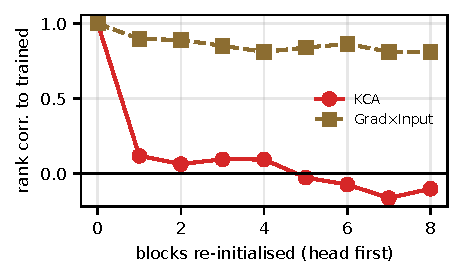
\includegraphics[width=0.85\linewidth]{fig/sanity.pdf}
\caption{Cascading model randomisation~\cite{adebayo2018sanity} of P4Transformer, from the classification head down: rank correlation of the attribution map with the trained model's.}
\label{fig:sanity}
\end{figure}

\begin{figure*}[p]
\centering
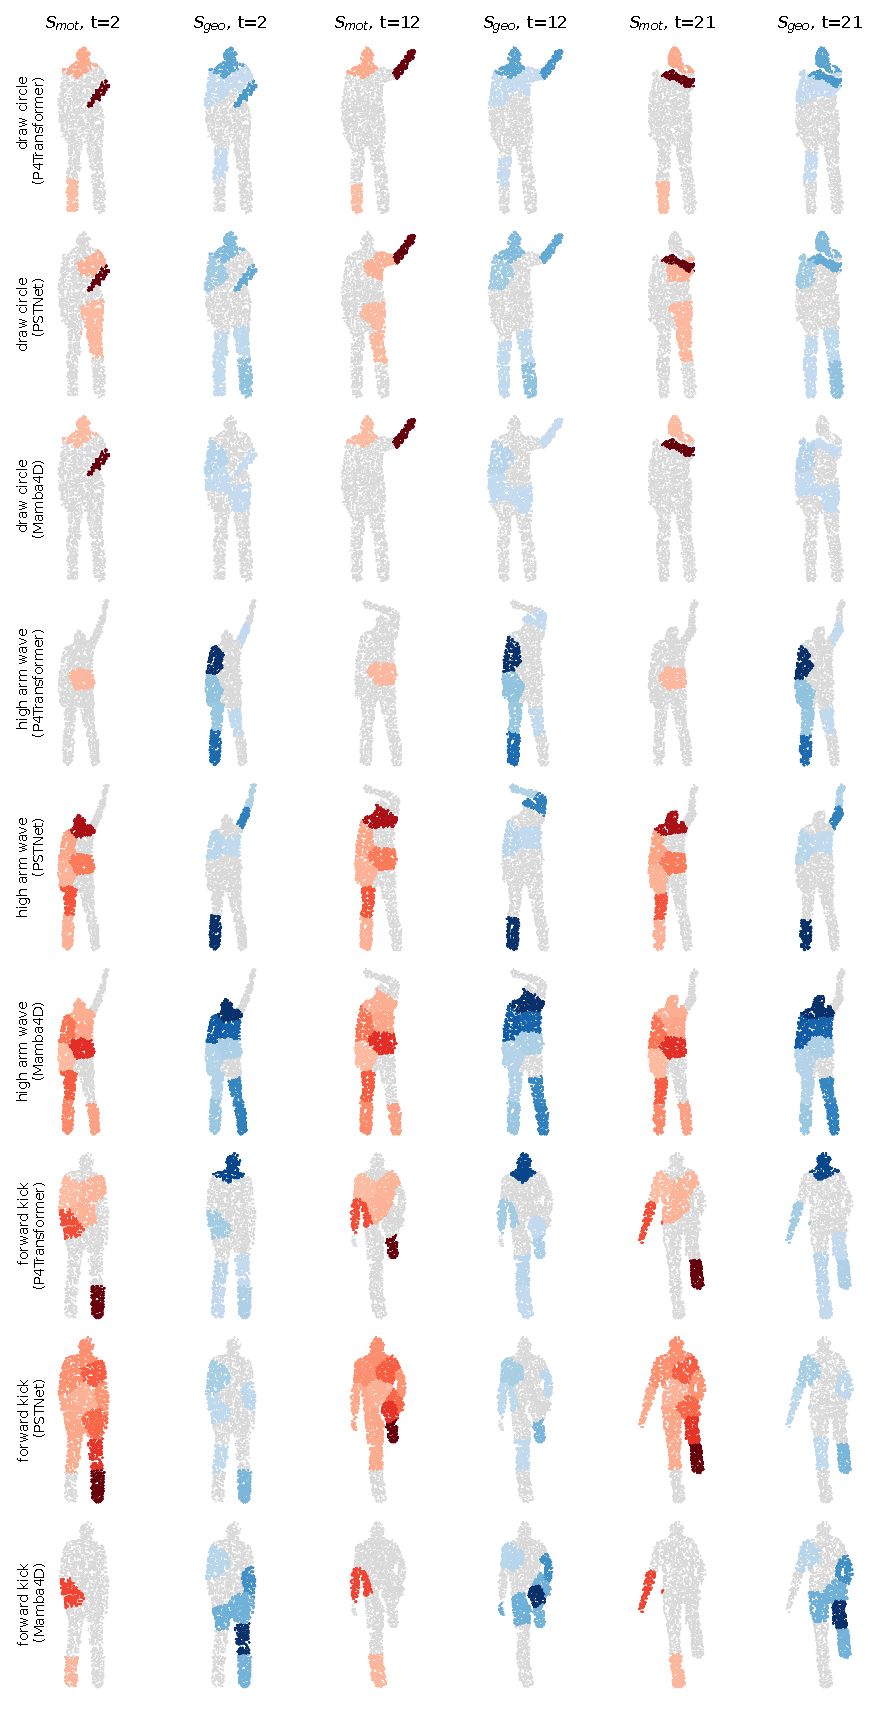
\includegraphics[width=\textwidth,height=0.92\textheight,keepaspectratio]{fig/msr_qual.pdf}
\caption{$\Smot$ (red) and $\Sgeo$ (blue) on real MSR-Action3D test clips at three instants; rows: three actions (\emph{draw circle}, \emph{high arm wave}, \emph{forward kick}) $\times$ the three backbones, same code.}
\label{fig:qual}
\end{figure*}

\begin{table}[h]
\centering\small\tablecitesoff\setlength{\tabcolsep}{3pt}
\begin{tabular}{l cccc}
\toprule
Action & mot.\ share & Del.\ \method & Del.\ occl. & acc.\,\%\\
\midrule
\tabinput{tables/tab_per_class.tex}
\bottomrule
\end{tabular}
\caption{Per action (P4Transformer, all test clips of each action): motion share $\Smot^+/(\Smot^++\Sgeo^+)$ of \method\ (context) over the whole body, deletion AUC of \method\ (context) and of region occlusion, and the model's accuracy on these clips.}
\label{tab:per-class}
\end{table}
